\begin{figure}[h!]
	\begin{center}
		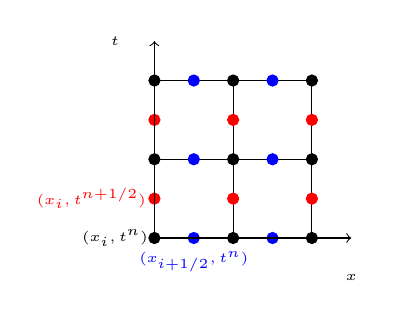
\begin{tikzpicture}

\draw[thin] (0, 0) grid (2, 2);
\foreach \x in {0,1,2}
	\foreach \y in {0,1,2}
		\draw[fill](\x,\y) circle (2pt) ;
\foreach \x in {0.5,1.5}
	\foreach \y in {0,1,2}
		\draw[fill,blue](\x,\y) circle (2pt) ;
\foreach \x in {0,1,2}
	\foreach \y in {0.5,1.5}
		\draw[fill,red](\x,\y) circle (2pt) ;		
 \draw[->] (0,0) -- (0,2.5);
  \draw[->] (0,0) -- (2.5,0);
      \coordinate (Origin)   at (0,0);
      \node (xlab) at (2.5,-0.5){\tiny $x$};
      \node (tlab) at (-0.5,2.5){\tiny $t$};
%      \node[black] (exux) at (2.6,1){\tiny $E_x$, $u_x$};
%      \node[blue](eyuy) at (1.5,2.5){\tiny $E_y$, $u_y$};
%      \node[red] (hz) at (2.5,1.5) {\tiny $H_z$};
      \node[black] (xilab) at (-0.5,0){\tiny $(x_i, t^n)$};
      \node[blue](xid) at (0.5,-0.3){\tiny $(x_{i+1/2},t^n)$};
      \node[red] (tid) at (-0.8,0.5) {\tiny $(x_i,t^{n+1/2})$};


		\end{tikzpicture} 
		\label{schemepos}
		\caption{Positions of $Ex$, $u_x$ (black dots), $E_y$ $u_y$ (blue dots) and $H_z$ (red dots) on the discretized grid in space and time}
	\end{center}
\end{figure}